

Let
\begin{align}
  \vec{M} &=  \myvec{\vec{A}-\vec{B}&\vec{B}-\vec{C}}^{\top}
% \end{align}
% where $rank(\vec{M})=1$.We have the matrix $\vec{M}$ as,
% \begin{align}
  & = \myvec{k-6&3-(-2)\\6-(-3)&-2-4} \\
  & =   \myvec{k-6&5\\9&-6}
\end{align}
Upon row reduction,
\begin{align}
\myvec{k-6&5\\9&-6}
\xleftrightarrow{R_1\leftrightarrow R_2}
\myvec{9&-6\\k-6&5}
% \\
% \leftrightarrow
% \myvec{9&-6\\0&9\times5-(-6\times(k-6))}
\\
\xleftrightarrow[]{}
\myvec{9&-6\\0&9+6k}
\\
\xleftrightarrow{R_2\rightarrow\frac{R_2}{6}}
\myvec{9&-6\\0&\frac{3}{2}+k}
\\
\xleftrightarrow{R_1\rightarrow \frac{R_1}{3}}
\myvec{1&\frac{-2}{3}\\0&\frac{3}{2}+k}
\end{align}
$\because$ the points are collinear, $\text{rank}(\vec{M})=1$.  Hence, 
\begin{align}
 \frac{3}{2}+k&=0 \\
\implies k&=\frac{-3}{2}
 \end{align}
This is verified in Fig.     \ref{vec/2008/14/Graphical solution}.
\begin{figure}[ht]
    \centering
    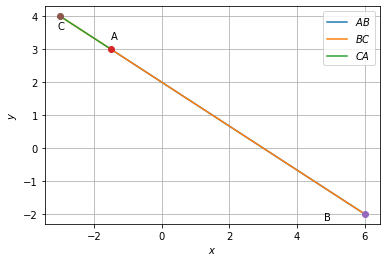
\includegraphics[width=\columnwidth]{vectors/solutions/2008/14/Collinear.png}
    \caption{Graphical solution}
    \label{vec/2008/14/Graphical solution}
\end{figure}



